\documentclass[text.tex]{subfiles}

\begin{document}

\section*{Delone set and voronoi tessellation}

Section provides the definitions of a delone set, a covering radius and a voronoi tessellation.

\begin{definition}
\label{def:delone}
Let $P\subset \mathbb{R}^n$ and $\exists R>0, \exists r>0$:
$$\forall x,y\in P,\, x\neq y: r\leq \|x-y\|$$
$$\forall z\in\mathbb{R}^n \exists x\in P: \|z-x\|\leq R$$
Then $P$ is called \textbf{delone} set.\\
For each delone set $P$ \textbf{covering radius} is defined as:
$$R_c = \inf\{R>0\,|\, z\in\mathbb{R}^n \exists x\in P: \|z-x\|\leq R\}$$
\end{definition}

\begin{definition}
Let $P\subset \mathbb{R}^n$, $P$ is a discrete set and $x\in P$. Then
$$V(x) = \left\{ y \in \mathbb{R}^n \,|\, \forall z \in P, z\neq x:\, \|y-x\|<\|y-z\| \right\}$$
is called \textbf{voronoi tile} (polygon) of $x$ on $P$.
\end{definition}

\begin{theorem}
\label{the:radiusLimit}
Let $P\subset \mathbb{R}^n$ is a delone set and $R_c$ it's covering radius. For any $x\in P$:
$$N_x = \{z\in P\,|\, z\neq x \wedge \|z-x\|\leq 2R_c\}$$
Then voronoi tile of $x$ on $P$ is
$$V(x) = \bigcap_{z\in \boldsymbol{N}} \left\{ y \in \mathbb{R}^n \,|\, \|y-x\|<\|y-z\| \right\}$$
\end{theorem}

\section{Two-dimensional quasicrystals}%=======================================================================================================================
\label{sec:twoDimension}
In the following section two-dimensional quasicrystal is defined and analyzed. Thanks to the Theorem \ref{the:twoToOne} analysis of one-dimensional quasicrystals can be in some way applied to the two-dimensional quasicrystals as well. 
\begin{definition}
Vectors $\alpha_1$, $\alpha_2$, $\alpha_3$ and the set $M$ denote the following.
$$\alpha_1 = \left( 1,0 \right) \quad \alpha_2 = \left( \frac{2-\beta}{2}, \frac{1}{2} \right) \quad \alpha_3 = \left( \frac{\beta-2}{2}, \frac{1}{2} \right)$$
$$M = \ring\alpha_1 + \ring\alpha_2$$
\end{definition}

\begin{remark}
The vectors and the set from previous definition are key to two-dimensional quasicrystal definition. The set $M$ is used as two-dimensional equivalent to $\ring$ from one-dimensional quasicrystal. Function from the following definition is used as two-dimensional equivalent to $'$.
\end{remark}

\begin{definition}
\label{def:starFunction}
Function $\ast: M \to M$ is called \textbf{star} function:
$$v^\ast = (a\alpha_1 + b\alpha_2)^\ast = a'\alpha_1 + b'\alpha_3 \;\forall a,b\in\ring$$
\end{definition}

\begin{remark}
Simple consequence of the Theorem \ref{def:starFunction} is $\alpha_1^\ast = \alpha_1$ and $\alpha_2^\ast = \alpha_3$.
\end{remark}

\begin{definition}
Let $\Omega \subset \mathbb{R}^2$ be bounded set with nonempty interior. Then \textbf{two-dimensional quasicrystal} with the window $\Omega$ is defined as:
$$\quasi{\Omega} = \left\{ x \in M\,|\,x^\ast \in \Omega \right\}$$
\end{definition}

\begin{remark}
$\quasi{\Omega}$ where $\Omega \subset \mathbb{R}^2$ always denotes two-dimensional quasicrystal.
\end{remark}

\begin{remark}
\label{rem:quasiProperties}
The same properties from the Theorem \ref{the:quasiProperties} for the one-dimensional quasicrystals apply to the two-dimensional quasicrystals as well.
\end{remark}

To analyze the two-dimensional quasicrystals again only windows of a certain shape will be considered. That is sufficient because of the Remark \ref{rem:quasiProperties}. The chosen window shape is a rhombus. 

\begin{theorem}
\label{the:twoToOne}
Let $I_1 = [c_1,d_1)$, then for the rhombus $\Omega = I\alpha_1^\ast + I\alpha_2^\ast$ and the quasicrystal $\quasi{\Omega}$: 
$$\quasi{\Omega} = \quasi{I}\alpha_1 + \quasi{I}\alpha_2$$
\end{theorem}

\begin{remark}
Note in previous theorem that while $\Omega \subset \RN^2$ and so $\quasi{\Omega}$ is a two-dimensional quasicrystal, $I \subset \RN$ and so $\quasi{I}$ is a one-dimensional quasicrystal. 
The same Theorem also applies to parallelogram shaped windows. 
\end{remark}

From the analysis of one-dimensional quasicrystals and Theorem \ref{the:twoToOne} follows that the two-dimensional quasicrystals are delone sets.  

To analyze distribution of the points of a two-dimensional quasicrystal, voronoi tessellation is used. The goal is to catalog shapes of all voronoi tiles that appear in a quasicrystal with a rhombus window. 

First an algorithm for generation of a finite section of a quasicrystal is presented. 

\section{Generation of a finite section of a quasicrystal with a rhombus window}
The algorithm is rather simple. It uses the stepping function and the Theorem \ref{the:twoToOne}. 

\paragraph{Algorithm definition} The algorithm receives as an input a rhombus window $\Omega = I\alpha_1^\ast + I\alpha_2^\ast$ and bounds $x_1, x_2, y_1, y_2 \in \ring$.
The algorithm returns a set of points from $\ring^2$ bounded by the given bounds.

First the one-dimensional interval $I = [c,d)$ needs to be scaled and moved in such a way, that it becomes a base window and contains $0$.
$$(\exists k\in\ZN)(\exists \lambda\in\ring) : \left(I = \beta^k\tilde{I}+\lambda\right) \wedge \left(|\tilde{I}| \in \left(\frac{1}{\beta},1\right] \right)\wedge \left(0\in\tilde{I}\right)$$

Now the stepping function can be used to iterate from 0 and generate enough points of the quasicrystal $\quasi{\tilde{I}}$ to cover the bounds. However since the bounds are for the quasicrystal $\quasi{\Omega}$ they also need to be transformed to be applicable to the quasicrystal $\quasi{\tilde{I}}$. 
\begin{align*}
\tilde{x_1} &= x_1 - (\beta-2)(y_2-y_1) & \tilde{y_1} &= 2y_1 \\
\tilde{x_2} &= x_2 & \tilde{y_2} &= 2y_2 
\end{align*}
The stepping function is then used to acquire two sections of the quasicrystal $\quasi{\tilde{I}}$: $\quasi{\tilde{I}}\cap[\tilde{x_1},\tilde{x_2}]$ and $\quasi{\tilde{I}}\cap[\tilde{y_1},\tilde{y_2}]$.

Each section needs to be transformed back:
$$\quasi{I} = \beta^k\quasi{\tilde{I}} + \lambda'$$
and finaly the finite section of the quasicrystal $\quasi{\Omega}$ is constructed:
$$\quasi{\Omega} = \quasi{I}\alpha_1 + \quasi{I}\alpha_2$$

\begin{figure}[h]
\centering
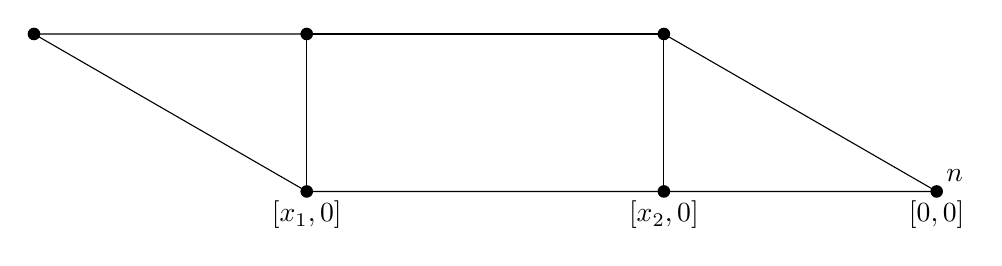
\begin{tikzpicture}[scale=4]
% nodes
\draw [-] (0,0)  -- (-2,0) -- (-2.86602540378,0.5) -- (-0.86602540378,0.5) -- cycle;
\draw [-] (-0.86602540378,0)  -- (-2,0) -- (-2,0.5) -- (-0.86602540378,0.5) -- cycle;

\fill (0,0) circle (0.02);
\fill (-2,0) circle (0.02);
\fill (-2.86602540378,0.5) circle (0.02);
\fill (-0.86602540378,0.5) circle (0.02);
\fill (-0.86602540378,0) circle (0.02);
\fill (-2,0.5) circle (0.02);

\node [below] at (0,0) {$[0,0]$};
\node [below] at (-0.86602540378,0) {$[x_2,0]$};
\node [below] at (-2,0) {$[x_1,0]$};
\node [above right] at (0,0) {$n$};

\end{tikzpicture}
\caption{Section of the artificial quasicrystal with the circumcircle and a circle of the estimated radius.}
\label{fig:coveringRadius}
\end{figure}

\begin{remark}
Due to the transformation of the bounds and the way the two-dimensional quasicrystal is constructed, the result will contain more points then requested. However the excess points can be easily discarded.
\end{remark}
\end{document}
